\section{Test of DALI Zensor 5}
This section will go through a test of a loudspeaker to understand how vibrations in the loudspeaker affect the distortion of the loudspeaker.
The loudspeaker which will be the basis for the test is the Zensor 5 (as seen on \autoref{fig:dali_zensor5}) given by DALI. A passive speaker has been choosen for the test because the amplifiers in DALI's active speakers are designed not to pressure the loudspeaker to its limits and beyond, and to be able to test how the vibrations affect distortion the loudspeaker must be tested to its limits and beyond.

\begin{figure}[H]
\centering
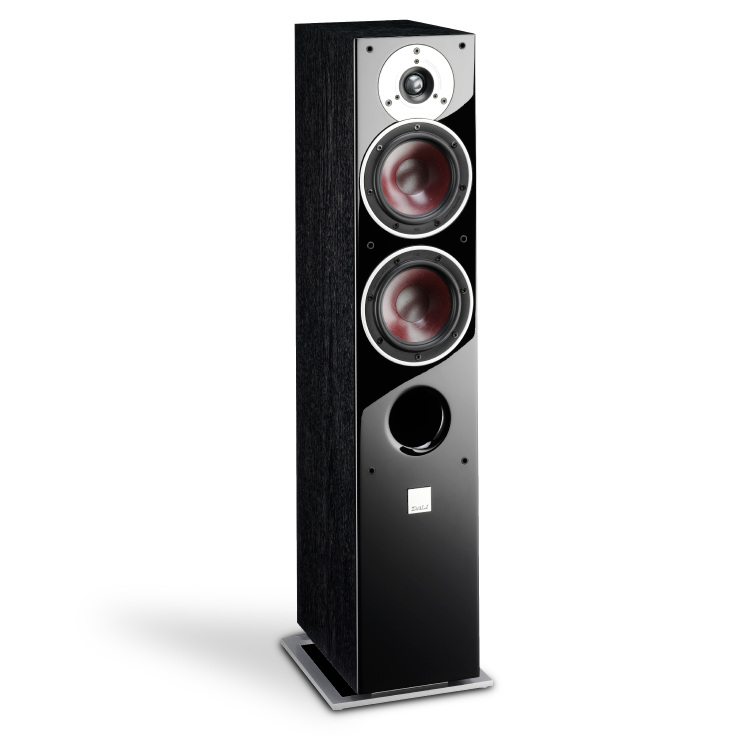
\includegraphics[width=0.5\textwidth]{figures/zensor5.png}
\caption{DALI zensor 5.}
\label{fig:dali_zensor5}
\end{figure}

\todo[inline]{Reference http://www.dali-speakers.com/loudspeakers/zensor/zensor-5/}

For measuring the vibrations inside the enclosure two accelometers have been placed inside the enclosure, one on the back of bottom driver and one on the top back of the enclosure. For measuring distortion a microphone has been placed 1 m from the speaker. To limit any reflection from a room for example, the test is perfomed in the Anechoic room at \gls{AAU} see  \todo[inline]{Reference http://doc.es.aau.dk/labs/acoustics/facilities/anechoic_room_large/} 



The loudspeaker is set to play a sinesweep from the crossover frequency of the speaker which is 2400 Hz to 10 Hz. The sine sweep is then repeated from the lowest volume setting of an 600 watt power amplifier until the loudspeaker breaks. This resulted in 20 sine sweep measurements from all three sensors which can be seen in the full test jounal in \autoref{app:journal_speaker_test}.      




